%--------------------------------------------------------------------
% NE 155 (intro to numerical simulation of radiation transport)
% Spring 2014

% formatting
\documentclass[12pt]{article}
\usepackage[top=1in, bottom=1in, left=1in, right=1in]{geometry}

\usepackage{setspace}
\onehalfspacing

\setlength{\parindent}{0mm} \setlength{\parskip}{1em}


% packages
\usepackage{amssymb}
%% The amsthm package provides extended theorem environments
\usepackage{amsthm}
\usepackage{epsfig}
\usepackage{times}
\renewcommand{\ttdefault}{cmtt}
\usepackage{amsmath}
\usepackage{graphicx} % for graphics files

% Draw figures yourself
\usepackage{tikz} 
\usetikzlibrary{petri}

% The float package HAS to load before hyperref
\usepackage{float} % for psuedocode formatting
\usepackage{xspace}

% from Denovo methods manual
\usepackage{mathrsfs}
\usepackage[mathcal]{euscript}
\usepackage{color}
\usepackage{array}

\usepackage[pdftex]{hyperref}

\newcommand{\nth}{n\ensuremath{^{\text{th}}} }
\newcommand{\ve}[1]{\ensuremath{\mathbf{#1}}}
\newcommand{\macro}{\ensuremath{\Sigma}}
\newcommand{\vOmega}{\ensuremath{\hat{\Omega}}}
\newcommand{\Macro}{\ensuremath{\Sigma}}

\newcommand{\cc}[1]{\ensuremath{\overline{#1}}}
\newcommand{\ccm}[1]{\ensuremath{\overline{\mathbf{#1}}}}


%--------------------------------------------------------------------
%--------------------------------------------------------------------
\begin{document}
\begin{center}
{\bf NE 155, Classes 27, 28, S14 \\
2-D Finite Difference/Volume methods\\ 
April 2 \& 4, 2014}
\end{center}

\setlength{\unitlength}{1in}
\begin{picture}(6,.1) 
\put(0,0) {\line(1,0){6.25}}         
\end{picture}


%-------------------------------------------------------------
\section{PDEs}

We'll start by considering PDEs in general, and then move on to the Diffusion Equation specifically.

A partial differential equation is an equation containing an unknown function of two or more variables and its derivatives with respect to those variables. 

If the PDE is linear in $u$ and all derivatives of $u$, then we say that the PDE is linear.
%
\begin{equation}
A\frac{\partial^2 u}{\partial x^2} + B\frac{\partial^2 u}{\partial x \partial  y} + C\frac{\partial^2 u}{\partial y^2} + D\frac{\partial u}{\partial x} + E\frac{\partial u}{\partial y} + Fu = G \nonumber
\end{equation}
%
This equation is a \textbf{2nd order} PDE in two variables. It is \textbf{linear} if $A$ through $G$ do not depend on $u$ (they may depend on $x$ and $y$).

%-------------------------------------------------------------
\vspace*{1em}

Recall that we can classify PDEs based on the geometric behavior of their solutions. \\
\underline{Note:} these classifications only apply to second order PDEs. 

\begin{itemize}
\item Elliptic if $B^2 - 4 AC < 0$. 

\item Hyperbolic if $B^2 - 4 AC > 0$

\item Parabolic if $B^2 - 4 AC = 0$
\end{itemize}

%-------------------------------------------------------------
\subsection{Elliptic Equations}

Recall that the 2-D Laplacian for the function$u(x,y)$ is
%
\begin{equation}
\nabla^2 u(x,y) = \frac{\partial^2 u}{\partial x^2} + \frac{\partial^2 u}{\partial y^2} = u_{xx} + u_{yy} \nonumber
\end{equation}
%
The Laplacian is used in many of the equations that are commonly found in physics:
%
\begin{itemize}
\item Laplace's equation
\[\nabla^2 u(x,y) = 0\]

\item Poisson's equation 
\[\nabla^2 u(x,y) = g(x,y)\]

\item Helmholtz's equation
\[\nabla^2 u(x,y) +f(x,y)u(x,y) = g(x,y)\]
\end{itemize}

% -----------------------------------------------------
\subsection{Meshing}

We will use 5 points to define our differenced Laplacian:

\begin{minipage}{0.5\textwidth}
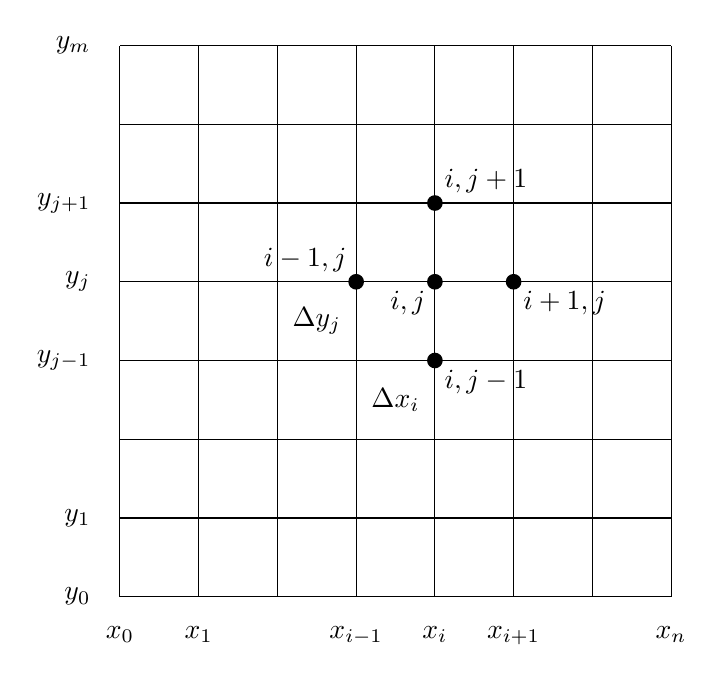
\begin{tikzpicture}
\draw (0,0)--(0,7);
\draw (1,0)--(1,7);
\draw (2,0)--(2,7);
\draw (3,0)--(3,7);
\draw (4,0)--(4,7);
\draw (5,0)--(5,7);
\draw (6,0)--(6,7);
\draw (7,0)--(7,7);
\node[below] at (0,-.25) {$x_0$};
\node[below] at (1,-.25) {$x_1$};
\node[below] at (3,-.25) {$x_{i-1}$};
\node[below] at (4,-.25) {$x_i$};
\node[below] at (5,-.25) {$x_{i+1}$};
\node[below] at (7,-.25) {$x_n$};
\node at (3.5, 2.5) {$\Delta x_i$};
% begin y
\draw (0,0)--(7,0);
\draw (0,1)--(7,1);
\draw (0,2)--(7,2);
\draw (0,3)--(7,3);
\draw (0,4)--(7,4);
\draw (0,5)--(7,5);
\draw (0,6)--(7,6);
\draw (0,7)--(7,7);
\node[left] at (-.25, 0) {$y_0$};
\node[left] at (-.25,1) {$y_1$};
\node[left] at (-.25,3) {$y_{j-1}$};
\node[left] at (-.25,4) {$y_j$};
\node[left] at (-.25,5) {$y_{j+1}$};
\node[left] at (-.25,7) {$y_m$};
  \node at (2.5,3.5) {$\Delta y_j$};
% labels
\node at (4,4) [circle,fill=black,scale=0.6] {};
\node[below left] at (4,4) {$i,j$};
\node at (5,4) [circle,fill=black,scale=0.6] {};
\node[below right] at (5,4) {$i+1,j$};
\node at (3,4) [circle,fill=black,scale=0.6] {};
\node[above left] at (3,4) {$i-1,j$};
\node at (4,5) [circle,fill=black,scale=0.6] {};
\node[above right] at (4,5) {$i,j+1$};
\node at (4,3) [circle,fill=black,scale=0.6] {};
\node[below right] at (4,3) {$i,j-1$};
\end{tikzpicture}
\end{minipage} \hfill
%
\begin{minipage}{0.5\textwidth}
  \[u(x_i,y_j) = u_{i,j} \qquad u(x_{i+1},y_j) = u_{i,j}\]
  \begin{align}
  \frac{\partial^2 u_{i,j}}{\partial x^2} = \frac{\partial}{\partial x}\bigl(\frac{\partial u_{i,j}}{\partial x}\bigr) =
\frac{u_{i-1,j} - 2u_{i,j} + u_{i+1,j}}{\Delta x_i^2} \nonumber \\
%
  \frac{\partial^2 u_{i,j}}{\partial y^2} = \frac{\partial}{\partial y}\bigl(\frac{\partial u_{i,j}}{\partial y}\bigr) =
\frac{u_{i,j-1} - 2u_{i,j} + u_{i,j+1}}{\Delta y_j^2} \nonumber
\end{align}
\end{minipage}

All together this gives
\[\nabla^2 u_{i,j} = 
\frac{\partial^2 u_{i,j}}{\partial x^2} + \frac{\partial^2 u_{i,j}}{\partial y^2} = 
\frac{u_{i-1,j} - 2u_{i,j} + u_{i+1,j}}{\Delta x_i^2} + \frac{u_{i,j-1} - 2u_{i,j} + u_{i,j+1}}{\Delta y_j^2}\]
%
If $\Delta x_i = $ constant $= \Delta y_j = h$, then
%
\[ \nabla^2 u_{i,j} = \frac{u_{i+1,j} + u_{i-1,j} + u_{i,j+1} + u_{i,j-1} - 4u_{i,j}}{h^2}\]

If we apply this to Laplace's equation and have fixed boundary conditions:
%
\begin{align}
u_{i+1,j} &+ u_{i-1,j} + u_{i,j+1} + u_{i,j-1} - 4u_{i,j} = 0 \:, i = 1, 2, \dots, n-1 \:, j = 1, 2, \dots, m-1 \nonumber \\
%
u_{0,j} &= BC_L \:, j = 1, 2, \dots, m-1 \nonumber \\
u_{i,0} &= BC_B \:, i = 1, 2, \dots, n-1 \nonumber \\
u_{n,j} &= BC_R \:, j = 1, 2, \dots, m-1 \nonumber \\
u_{i.m} &= BC_T \:, i = 1, 2, \dots, n-1 \nonumber
\end{align}
%
And make sure to check how the corners need to be defined. We could apply this directly the the 2-D diffusion equation.

%--------------------------------------------------------------------
\section{2-D Finite Volume Method, Diffusion Equation}

Remember that in 1-D we were solving this
\[-\frac{d}{dx}D(x)\frac{d \phi(x)}{dx} + \Sigma_a(x) \phi(x) = S(x)\]
%
with an equilibrium (reflecting) condition at the centerline ($x_0 = 0$) and vacuum on the right ($x_n = a$):
\begin{align}
\frac{d}{dx}\phi(x) \big|_{x=0} &= 0 \qquad \text{zero net current} \nonumber\\
\phi(\tilde{a}) &= 0 \qquad \tilde{a} = a + 2D \nonumber
\end{align}

We imposed a spatial mesh and said material discontinuities will coincide with the cell edges, $x_i$. Thus, we can assume that the cross sections and the diffusion coefficient are constant in each cell:
%
\begin{align}
D(x) &= D_i \qquad \text{for } x_{i-1} \leq x_i \nonumber \\
\Sigma_{a}(x) &= \Sigma_{a,i} \qquad \text{for } x_{i-1} \leq x_i \nonumber \\
h_i &\equiv x_i - x_{i-1} \nonumber 
\end{align}
%
The unknown fluxes and known sources are defined at the mesh or cell edges:
\begin{align}
\phi(x_i) &= \phi_i \nonumber \\
S(x_i) &= S_i \nonumber 
\end{align}
%
We then went on to define things for the finite volume method
\begin{center}
\begin{figure}[h!]
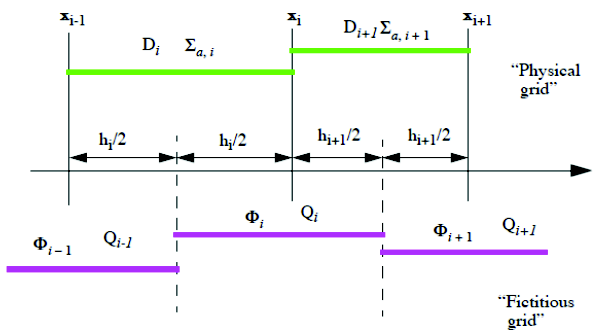
\includegraphics[height=2.5in]{FVM-DE}
\end{figure}
\end{center}

Now, we're going to extend all of this to two dimensions. We'll start with the multi-D equation:
\[-\nabla \cdot \bigl(D(\vec{r})\nabla \phi(\vec{r})\bigr) + \Sigma_a(\vec{r}) \phi(\vec{r}) = S(\vec{r})\]
%
This equation is elliptic:
\begin{itemize}
\item in general, this is the Helmholtz equation.
\item if $\Sigma_a(\vec{r})=0$ and $D(\vec{r})=$ constant, then this takes the form of the Poisson equation.
\item if $\Sigma_a(\vec{r})=0$ and $S(\vec{r})=0$, then this becomes Laplace's equation. 
\end{itemize}

In 2-D:
\[-\frac{\partial}{\partial x}D(x,y)\frac{\partial}{\partial x} \phi(x,y) + \Sigma_a(x,y) \phi(x,y) = S(x,y)\]
%
For now we're going to say we have fixed boundary conditions:
\[\phi(-a,y) = \Phi_L\:, \quad \phi(a,y) = \Phi_R\:, \quad \phi(x,-b) = \Phi_B\:, \quad \phi(x,b) = \Phi_T\:.\]
with $x \in [-a,a]$ and $y \in [-b,b]$.


% ---------------------------------------------------------
% ---------------------------------------------------------
\subsection{Finite Volume}

\begin{figure}[h!]
\begin{center}
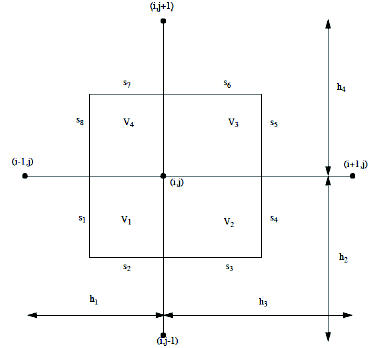
\includegraphics[height=5in]{2DfvmGrid}
\end{center}
\end{figure}

We assume the diffusion coefficient, absorption cross section, and source are constant in each cell (cell-centered), e.g., for $V_1$:
\begin{align}
D(x,y) &= D_{1}\;, \qquad x_{i-1} \leq x \leq x_i \:\text{ and }\: y_{j-1} \leq y \leq y_j \nonumber \\
%
\Sigma_a(x,y) &= \Sigma_{a,1}\;, \qquad x_{i-1} \leq x \leq x_i \:\text{ and }\: y_{j-1} \leq y \leq y_j \nonumber \\
%
S(x,y) &= S_{1}\;, \qquad x_{i-1} \leq x \leq x_i \:\text{ and }\: y_{j-1} \leq y \leq y_j \nonumber \\
%
h_1 &\equiv x_{i} - x_{i-1} \nonumber 
\end{align}
And analogously for the other 3 volumes.

We further assume that the fluxes are constant over the interval centered around $(x_i, y_j)$ (edge-centered):
%
\[\phi(x,y) = \phi_{i,j} \qquad \text{for } \bigl(x_i - \frac{h_1}{2}\bigr) \leq x \leq \bigl(x_i + \frac{h_{3}}{2}\bigr) \:\text{ and }\:\bigl(y_j - \frac{h_2}{2}\bigr) \leq x \leq \bigl(y_j + \frac{h_{4}}{2}\bigr) \]

Now, we integrate the 2-D equation over 4 rectangular volumes (well, areas, technically): $V = V_1 + V_2 + V_3 + V_4$.
%
\[\int_V d\vec{r}\:\bigl[-\nabla \cdot \bigl(D(\vec{r})\nabla \phi(\vec{r})\bigr)\bigr] + \int_V d\vec{r}\:\Sigma_a(\vec{r}) \phi(\vec{r}) = \int_V d\vec{r}\:S(\vec{r})\]


% ---------------------------------------------------------
\subsubsection{Streaming Term}
Use Gauss Theorem to replace the first volume integral with a surface integral:
%
\begin{align}
-\int_V d\vec{r}\:\bigl[\nabla \cdot \bigl(D(\vec{r})\nabla \phi(\vec{r})\bigr)\bigr] &= -\int_S d\vec{S} \cdot\bigl(D(\vec{r})\nabla \phi(\vec{r})\bigr) \nonumber \\
%
= -\int_S d\vec{S}\: D(\vec{r})\hat{n} \cdot \nabla \phi(\vec{r}) &= -\int_S d\vec{S} \:D(\vec{r})\frac{\partial}{\partial \hat{n}}\phi(\vec{r}) \nonumber
\end{align}
%
Next, we define the partial derivative w.r.t.\ direction on each surface, using $O(h)$ forward and backward difference schemes since they're simple:
\begin{align}
\frac{\partial}{\partial \hat{n}}\phi(\vec{r}) &= \frac{\phi_{i,j-1} - \phi_{i,j}}{h_2} \qquad \text{on } S_2 \:, S_3 \nonumber \\
%
&= \frac{\phi_{i,j+1} - \phi_{i,j}}{h_4} \qquad \text{on } S_7 \:, S_6 \nonumber \\
%
&= \frac{\phi_{i-1,j} - \phi_{i,j}}{h_1} \qquad \text{on } S_1 \:, S_8 \nonumber \\
%
&= \frac{\phi_{i+1,j} - \phi_{i,j}}{h_3} \qquad \text{on } S_4 \:, S_5 \nonumber 
\end{align}
%
We then use the midpoint rule for the integration and integrate along each surface. Recall that the physics values are cell-centered while the flux is edge-centered. E.g., surfaces $S_2$ and $S_3$:
%
\[-\int_{S_2+S_3} d\vec{S} \:D(\vec{r})\frac{\partial}{\partial \hat{n}}\phi(\vec{r}) = \boxed{\frac{\phi_{i,j} - \phi_{i,j-1}}{h_2} \biggl(\frac{D_1 h_1 + D_2 h_3}{2}\biggr)}\:,\]
%
and we do this for each set of surfaces. 


% ---------------------------------------------------------
\subsubsection{Absorption Term}
To integrate absorption, we do 4 integrals - one over each sub-volume:
%
\begin{align}
\int_{x_i-\frac{h_1}{2}}^{x_i+\frac{h_3}{2}} dx \int_{y_j-\frac{h_2}{2}}^{y_j+\frac{h_4}{2}}dy\:\Sigma_a(x,y) \phi(x,y) &= \Sigma_{a,1}\int\int_{V_1} dx dy \: \phi(x,y) + \nonumber \\
%
\Sigma_{a,2}\int\int_{V_2} dx dy \: \phi(x,y) &+ \Sigma_{a,3}\int\int_{V_3} dx dy \: \phi(x,y) + \Sigma_{a,4}\int\int_{V_4} dx dy \: \phi(x,y) \:.\nonumber
\end{align}
%
Again applying the midpoint scheme and using our edge-centered flux definition:
%
\[ \int \int dx dy\:\Sigma_a(x,y) \phi(x,y) = \boxed{\phi_{i,j}\bigl(\Sigma_{a,1} V_1 + \Sigma_{a,2} V_2 + \Sigma_{a,3} V_3 + \Sigma_{a,4} V_4 \bigr) }\:, \]
%
where
\[V_1 = \frac{1}{4}h_1h_2\:, \quad V_2 = \frac{1}{4}h_3h_2\:, \quad V_3 = \frac{1}{4}h_3h_4 \:, \quad V_4 = \frac{1}{4}h_1h_4 \:.\]


% ---------------------------------------------------------
\subsubsection{Source Term}
Using the same procedure for the source, we get:
\[\int \int dx dy \: \:S(x,y) = \boxed{ S_1 V_1 + S_2 V_2 + S_3 V_3 + S_4 V_4 }\:.\]


% ---------------------------------------------------------
\subsubsection{Discretized Equations}
Collecting all of the terms and separating them, we get a 5-point difference equation for $i=1,\dots,n-1$; $j=1,\dots,m-1$:
%
\[a_{i-1,j}\phi_{i-1,j} + a_{i+1,j}\phi_{i+1,j} + a_{i,j-1}\phi_{i,j-1} + a_{i,j+1}\phi_{i,j+1} + + a_{i,j}\phi_{i,j} = S_{i,j} \]
%
\begin{align}
a_{i-1,j} &= -\frac{D_1 h_2 + D_4 h_4}{2h_1} \nonumber \\
a_{i+1,j} &= -\frac{D_2 h_2 + D_3 h_4}{2h_3} \nonumber \\
a_{i,j-1} &= -\frac{D_1 h_1 + D_2 h_3}{2h_2} \nonumber \\
a_{i,j+1} &= -\frac{D_4 h_1 + D_4 h_1}{2h_4} \nonumber \\
%
a_{i,j} &= \sum_{k=1}^4 \Sigma_{a,k}V_k - \bigl(a_{i-1,j} + a_{i+1,j} + a_{i,j-1} + a_{i,j+1} \bigr)\nonumber \\
%
S_{i,j} &= \sum_{k=1}^4 S_{k}V_k \:.\nonumber
\end{align}


%-------------------------------------------------------
\subsection{Boundary Conditions}

When we're at the edges, we get 4 entries rather than 5 because the edge values are know. For corners we have only 3 entries. 

Let's see how this impacts our equations. Recall:
%
\[\phi(-a,y) = \Phi_L\:, \quad \phi(a,y) = \Phi_R\:, \quad \phi(x,-b) = \Phi_B\:, \quad \phi(x,b) = \Phi_T\:.\]
%
Let's choose what to do at the corners, and then define the rest of the boundaries:
\[\phi_{0,0} = \Phi_B\:, \quad \phi_{0,m} = \Phi_R\:, \quad \phi_{0,m} = \Phi_L\:, \quad \phi_{n,m} = \Phi_T\:.\]
%
\begin{align}
\phi_{0,j} &= \Phi_L \qquad j=1,\dots,m-1 \nonumber \\
\phi_{n,j} &= \Phi_R \qquad j=1,\dots,m-1 \nonumber \\
\phi_{i,0} &= \Phi_B \qquad i=1,\dots,n-1 \nonumber \\
\phi_{i,m} &= \Phi_T \qquad i=1,\dots,n-1 \nonumber \\
\end{align}

Let's look at how this would impact the left ($i=0$) boundary. The $i=0$ equations are simply the boundary condition and the $i=1$ equations become:
\[a_{i+1,j}\phi_{i+1,j} + a_{i,j-1}\phi_{i,j-1} + a_{i,j+1}\phi_{i,j+1} + + a_{i,j}\phi_{i,j} = S_{i,j} - a_{0,j}\phi_R \:.\]

To write the system in a way that looks like $\ve{A}\vec{x} = \vec{b}$, we need to choose an ordering strategy for how we want to store the points


\begin{minipage}{0.5\textwidth}
%-------------- indices ------------------
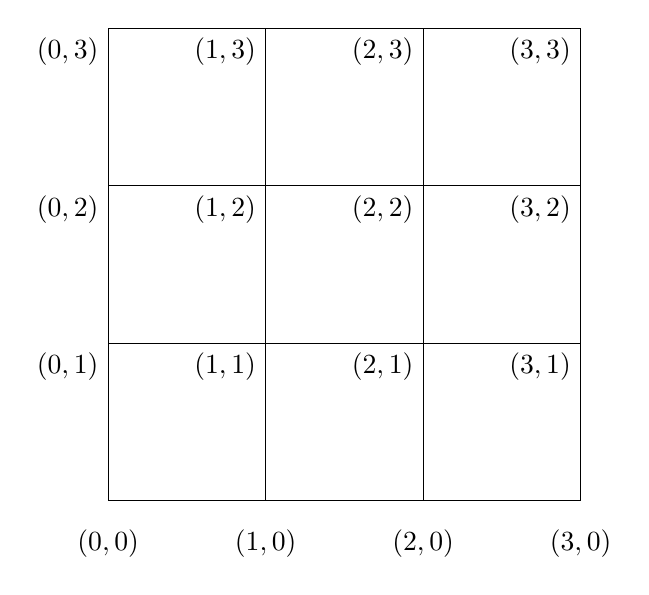
\begin{tikzpicture}
\draw[step=2cm] (0,0) grid (6,6);
\foreach \y in {1, 2, 3}
    \foreach \x in  {0, 1, 2, 3}
        \node[below left] at (2*\x cm,2*\y cm) {$(\x,\y)$};
\node[below] at (0,-.25) {$(0,0)$};
\node[below] at (2,-.25) {$(1,0)$};
\node[below] at (4,-.25) {$(2,0)$};
\node[below] at (6,-.25) {$(3,0)$};
\end{tikzpicture}
\end{minipage} \hfill
%-------------- numbered nodes ------------------
\begin{minipage}{0.5\textwidth}
\begin{tikzpicture}
\draw[step=2cm] (0,0) grid (6,6);
\node[below] at (0,-.25) {$0$};
\node[below] at (2,-.25) {$1$};
\node[below] at (4,-.25) {$2$};
\node[below] at (6,-.25) {$3$};
\node[below left] at (-.25,2) {$4$};
\node[below left] at (2,2) {$5$};
\node[below left] at (4,2) {$5$};
\node[below left] at (6,2) {$6$};
\node[below left] at (-.25,4) {$7$};
\node[below left] at (2,4) {$8$};
\node[below left] at (4,4) {$9$};
\node[below left] at (6,4) {$10$};
\node[below left] at (-.25,6) {$11$};
\node[below left] at (2,6) {$12$};
\node[below left] at (4,6) {$13$};
\node[below left] at (6,6) {$14$};
\end{tikzpicture}
\end{minipage}

%and the last equation for $i=n-1$ becomes
%\[a_{n-1,n-2} \phi_{n-2} + a_{n-1,n-1}\phi_{n-1} + a_{n-1, n} \times 0 = S_{n-1}\]
%
%Next we'll worry about the \textbf{reflecting} or zero current condition. The first step is to integrate over $[0, h_{1}/2]$.
%%
%\begin{figure}[h!]
%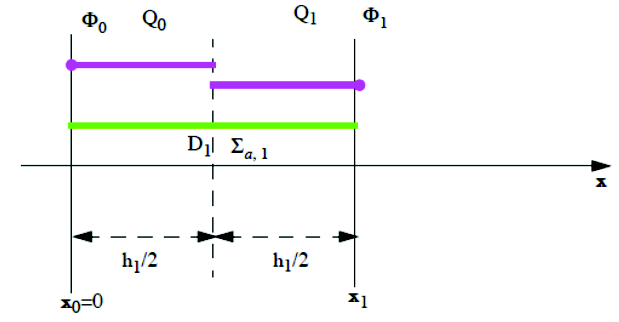
\includegraphics[height=2in]{ReflectingBC}
%\end{figure}
%%
%\begin{align}
%\int_{0}^{\frac{h_{1}}{2}} \biggl(-\frac{d}{dx}D(x)\frac{d \phi(x)}{dx}\biggr) dx &+ \int_{0}^{\frac{h_{1}}{2}} \Sigma_a(x) \phi(x) dx = \int_{0}^{\frac{h_{1}}{2}} S(x) dx \nonumber \\
%%
%-D(x)\frac{d \phi(x)}{dx}\big|_{\frac{h_{1}}{2}} &+ D(x)\frac{d \phi(x)}{dx}\big|_{0} + \Sigma_{a,1}\phi_0 \frac{h_1}{2} = S_0 \frac{h_1}{2} \nonumber 
%\end{align}
%%
%Now we can apply the boundary condition $\frac{d \phi(x)}{dx}\big|_{0} = 0$ to get:
%\[-D(x)\frac{d \phi(x)}{dx}\big|_{\frac{h_{1}}{2}} + \Sigma_{a,1}\phi_0 \frac{h_1}{2} = S_0 \frac{h_1}{2}\]
%
%And the first equation ($i=0$) becomes
%\[a_{00}^*\phi_0 + a_{01}^* \phi_1 = S_0\:,\]
%%
%where we redefine the $a$s to be (I've added the * to indicate that these have different definitions than the rest of the terms.)
%%
%\begin{align}
%a_{00}^* &= \frac{2D_1}{h_1^2} + \Sigma_{a,1} \nonumber \\
%a_{01}^* &= -\frac{2D_1}{h_1^2} \nonumber 
%\end{align}
%
%We now have $n$ equations and $n$ unknowns
%\begin{equation}
%\underbrace{\begin{pmatrix}
%a_{00}^* & a_{01}^* & 0      & 0 & \cdots & 0 \\
%a_{10}   & a_{11}   & a_{12} & 0 & \cdots & 0 \\
%0        & a_{21}   & a_{22}   & a_{23} &  & \vdots \\
%\vdots        &    & \ddots  & \ddots & \ddots & \vdots \\
%0 & \cdots & 0 & a_{n-3,n-3}   & a_{n-2,n-2} & a_{n-2,n-1} \\
%0        & \cdots   & 0   & 0 & a_{n-1,n-2} & a_{n-1,n-1} 
%\end{pmatrix}}_{\ve{A}}
%%
%\underbrace{\begin{pmatrix}\phi_0 \\ \phi_1 \\ \phi_2 \\ \vdots \\ \phi_{n-2} \\ \phi_{n-1} \end{pmatrix}}_{\vec{\phi}} =
%%
%\underbrace{\begin{pmatrix}S_0 \\ S_1 \\ S_2 \\ \vdots \\ S_{n-2} \\ S_{n-1} \end{pmatrix}}_{\vec{S}}
%\end{equation}




%--------------------------------------------------------------------
%--------------------------------------------------------------------
%\bibliographystyle{plain}
%\bibliography{LinearSolns} 

\end{document}